\documentclass[
  bibliography=totoc,     % Literatur im Inhaltsverzeichnis
  captions=tableheading,  % Tabellenüberschriften
  titlepage=firstiscover, % Titelseite ist Deckblatt
]{scrartcl}

% LaTeX2e korrigieren.
\usepackage{fixltx2e}
% Warnung, falls nochmal kompiliert werden muss
\usepackage[aux]{rerunfilecheck}

% deutsche Spracheinstellungen
\usepackage{polyglossia}
\setmainlanguage{german}
% \usepackage{german}


% unverzichtbare Mathe-Befehle
\usepackage{amsmath}
% viele Mathe-Symbole
\usepackage{amssymb}
% Erweiterungen für amsmath
\usepackage{mathtools}

% Fonteinstellungen
\usepackage{fontspec}

\defaultfontfeatures{Ligatures=TeX}

\usepackage[
  math-style=ISO,    % \
  bold-style=ISO,    % |
  sans-style=italic, % | ISO-Standard folgen
  nabla=upright,     % |
  partial=upright,   % /
]{unicode-math}

\setmathfont{Latin Modern Math}
\setmathfont[range={\mathscr, \mathbfscr}]{XITS Math}
\setmathfont[range=\coloneq]{XITS Math}
\setmathfont[range=\propto]{XITS Math}
% make bar horizontal, use \hslash for slashed h
\let\hbar\relax
\DeclareMathSymbol{\hbar}{\mathord}{AMSb}{"7E}
\DeclareMathSymbol{ℏ}{\mathord}{AMSb}{"7E}

% richtige Anführungszeichen
\usepackage[autostyle]{csquotes}

% Zahlen und Einheiten
\usepackage[
  locale=DE,                   % deutsche Einstellungen
  separate-uncertainty=true,   % Immer Fehler mit \pm
  per-mode=symbol-or-fraction, % m/s im Text, sonst Brüche
]{siunitx}

% chemische Formeln
\usepackage[version=3]{mhchem}

% schöne Brüche im Text
\usepackage{xfrac}

% Floats innerhalb einer Section halten
\usepackage[section, below]{placeins}
% Captions schöner machen.
\usepackage[
  labelfont=bf,        % Tabelle x: Abbildung y: ist jetzt fett
  font=small,          % Schrift etwas kleiner als Dokument
  width=0.9\textwidth, % maximale Breite einer Caption schmaler
]{caption}
% subfigure, subtable, subref
\usepackage{subcaption}

% Grafiken können eingebunden werden
\usepackage{graphicx}
% größere Variation von Dateinamen möglich
\usepackage{grffile}

% Standardplatzierung für Floats einstellen
\usepackage{float}
\floatplacement{figure}{htbp}
\floatplacement{table}{htbp}

% schöne Tabellen
\usepackage{booktabs}

% Seite drehen für breite Tabellen
\usepackage{pdflscape}

% Literaturverzeichnis
\usepackage[backend=biber]{biblatex}
% Quellendatenbank
\addbibresource{lit.bib}
\addbibresource{programme.bib}

% Hyperlinks im Dokument
\usepackage[
  unicode,
  pdfusetitle,    % Titel, Autoren und Datum als PDF-Attribute
  pdfcreator={},  % PDF-Attribute säubern
  pdfproducer={}, % "
]{hyperref}
% erweiterte Bookmarks im PDF
\usepackage{bookmark}

% Trennung von Wörtern mit Strichen
\usepackage[shortcuts]{extdash}

\usepackage{multicol}



\author{
  Falko Barth
  \texorpdfstring{
    \\
    \href{mailto:andreas.farenbruch@udo.edu}{falko.barth@udo.edu}
  }{}%
  \texorpdfstring{\and}{, }
  Egor Evsenin-Gutschank
  \texorpdfstring{
    \\
    \href{mailto:egor.evsenin@udo.edu}{egor.evsenin@udo.edu}
  }{}
}
\publishers{TU Dortmund – Fakultät Physik}

\titlehead{
\includegraphics[height=1.5cm]{logos/tu-logo.pdf}}

%%% Hier definiert man Titel, Autor und Datum %%%%%%%%%%%%%%%%%%%%%%%%%%%%%%%%%

\subject{Versuch Nr.48}
\title{Debye-Scherrer-Aufnahmen}
\date{
  Durchführung: 29.10.2018
  \hspace{3em}
  Abgabe: 01.11.2018
}

%%%%%%%%%%%%%%%%%%%%%%%%%%%%%%%%%%%%%%%%%%%%%%%%%%%%%%%%%%%%%%%%%%%%%%%%%%%%%%%

\begin{document}

\maketitle
\thispagestyle{plain}
%\leftmark{TU Dortmund -Fakultät Physik}
\tableofcontents
\newpage

\section{Einleitung}
\label{sec:Einleitung}
In diesem Versuch werden kristalline Festkörper mit der Debye-Scherrer Methode untersucht. 
Der größte Teil der festen Materie ist kristallin. 
Sie zeichnet sich durch eine räumlich periodische Gitterstruktur aus, die sich makroskopisch fortsetzt. 
Die Unterschiede in der Struktur äußern sich in Anisitropen Eigenschaften der Gitterstruktur  und des Atomaren Aufbaus, wie zum Beispiel Elastizität und Permeabilität, die durch Tensor und Vektorfelder im Kristall hervorgerufen werden.\\
Es ist zwischen Einkristallen und Polykristallinen zu unterscheiden. 
Metalle sind polykristallin, so wie fast alle natürlich vorkommenden Kristalline.
Die daraus resultierenden makroskopischen Eigenschaften sind isotrop ergeben sich aus der Mittelung aller Kristallrichtungen im Festkörper.
Zur genauen Untersuchung der periodischen Struktur und inneren Ordnung sind Einkristalle notwendig.  
Diese Einkristalle werden mit Röntgenstrahlung, welche eine Wellenlänge im Bereich Angström besitzt, bestrahlt, damit diese an dem Festkörper gebeugt werden kann.
Ein Angström entspricht der Größenordnung der Gitterabstände der Atome, welche mit der Debye-Scherrer Methode bestimmt werden soll.	
\section{Theoretischer Hintergrund}
\label{sec:Theorie}
\subsection{Grundlegende Beschreibung von Kristallstrukturen}
Kristalle sind räumlich periodische Gitter, die durch die Verbindung der zugrunde liegenden Materialien besteht. 
Die kleinste Einheit dieses Gitters wird Basis genannt, welche durch drei Gittervektoren $\vec{a}$, $\vec{b}$ und $\vec{c}$ aufgespannt wird.
Die Struktur des Gitters ist durch die Basis dann eindeutig festgelegt und heißt Elementarzelle.
Ohne weitere Eigenschaften festzulegen gibt es unendlich viele Punktgitter.
Zwei 2D-Gitter sind in Abbiildung \ref{fig:2dgitter} dargestellt.
\begin{figure}
	\centering
	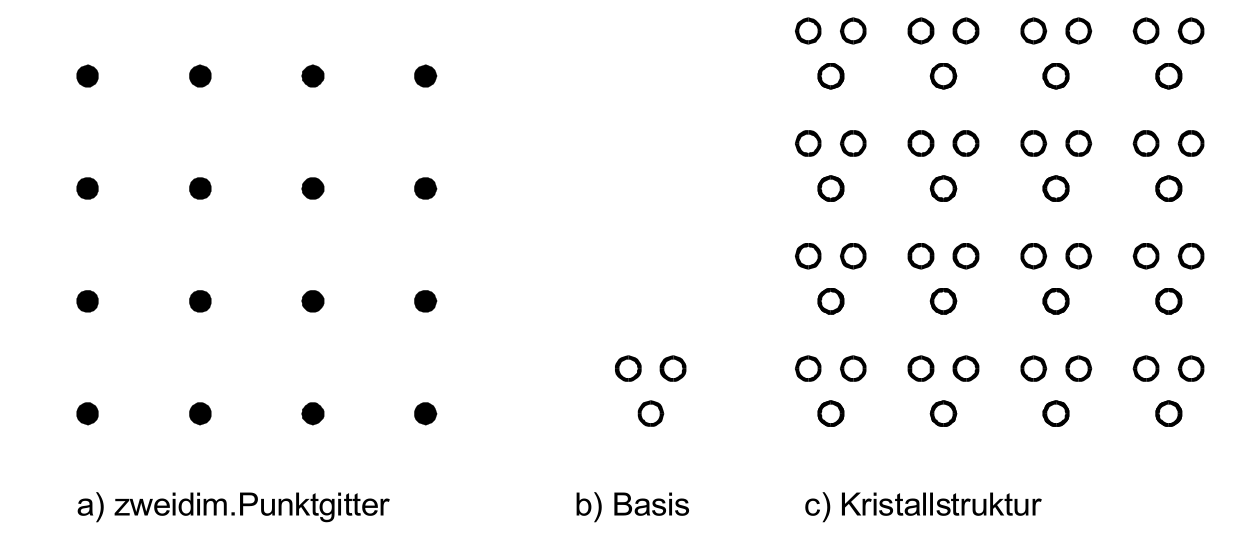
\includegraphics[width = \textwidth]{Abbildungen/2dgitter.png}
	\caption{Zeigt die Unterschiede zwischen Gitter, Basis und Kristallstruktur \cite{Anleitung}.}
	\label{fig:2dgitter}
\end{figure} 
Damit die Gitter klassifiziet werden können, wird die Invarianz unter Symmetrieeigenschaften getestet. \\
Die einfachste erhaltene Symmetrie, die einen Kristall auszeichnet ist die fundamentale Translation. Das bedeuetet, dass ein Vektor $\vec{t}$ durch die folgende Bedingung in Gleichung \ref{eq:fundamentale trans} aus den Basisvektoren darstellbar ist.
\begin{equation}
\vec{\text{t}} = n_1 \vec{\text{a}}+n_2 \vec{\text{b}}+n_3 \vec{\text{c}}
\label{eq:fundamentale trans}
\end{equation}
Die Vorfaktoren der Basisvektoren sind Elemente der natürlichen Zahlen $\mathbb{N}$.
Beistzt das Parallelepiped, welches durch die drei Basisvektoerne aufgespannt wird, nur in jeder Ecke ein Atom, so wird diese Zelle primitiv gennant.
Da nur der Anteil des Atoms, der innerhlab des Epipeds liegt, zählt, besteht die primitive EInheistzelle aus einem Atom.
Das ist die simpelste Form einer Zelle. 
Die weiteren Punktgitter, die durch die Symmetrieoperationen der Inversion, Spiegelung und Rotation klassifiziert werden, teilen sich in 14 Gittertypen auf. 
Diese heißen Bravais-Gitter und können in sieben Kristallsysteme, wie in Abbildung \ref{fig:System} unterteilt werden.
\begin{figure}
	\centering
	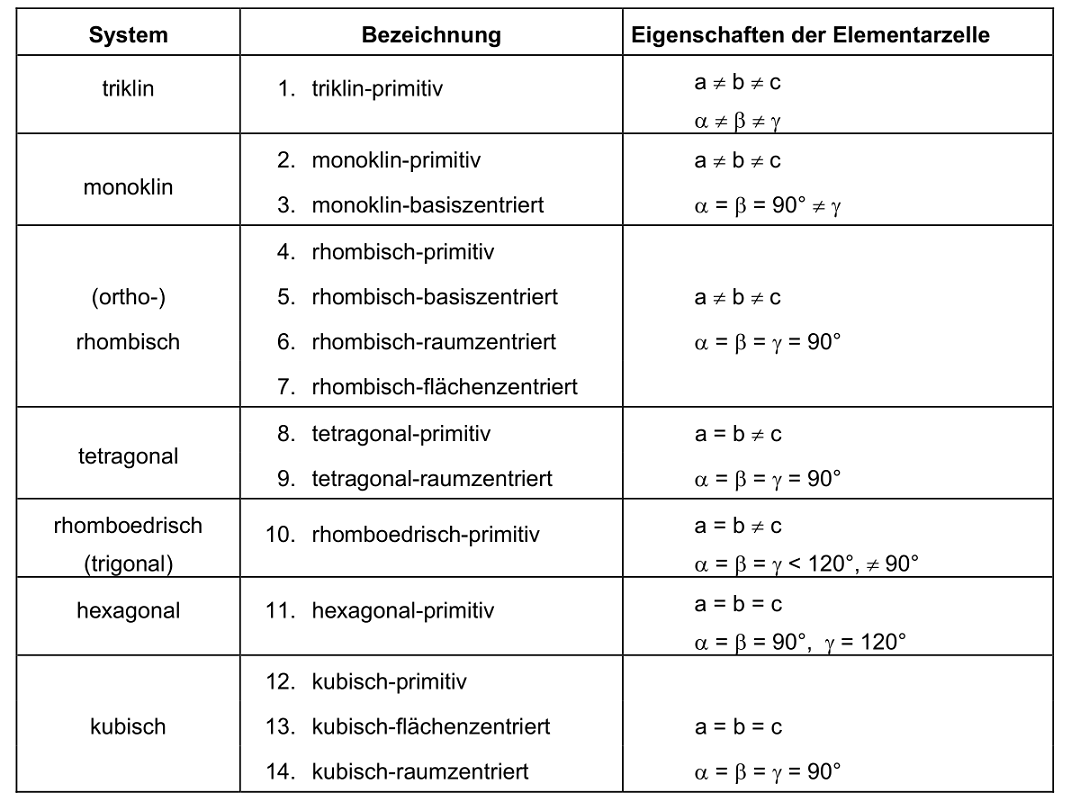
\includegraphics[width = \textwidth]{Abbildungen/System.png}
	\caption{Die Bravais-Gitter aufgeteilt in ihre Kristallsysteme mit den dazugehörigen Eigenschaften \cite{Anleitung}}
	\label{fig:System}
\end{figure} 
\subsection{Das kubische Kristallsystem}
Für die in diesem Versuch untersuchten Materialien ist insbesondere die kubische Gitterstruktur relvant, da Metalle und Salze vorzugsweise kubisch aufgebaut sind.
Das kubische System ist in drei Klassen eingeteilt.\\
Die simpelste Struktur weist das kubisch primitive Gitter auf, welches aus einem Atom besteht und die primitive Einheitszelle in Würfelform beschreibt.
Aus zwei Atomen pro Einheitszelle besteht das kubisch raumzentrierte Gitter, welches als Grundmodell die primitive Einheitszelle besitzt und zusätzlich in der Mitte des Würfels noch ein weiteres Atom besitzt.
Doppelt so viele Atome wie die das kubisch-raumzentrierte Gitter besitzt das kubisch-flächenzentrierte Gitter.
Hier liegt bei dem einfach kubische Gitter auf jeder Würfelfläche noch ein weiteres Atom.
Beispiele für die zuletzt genannten Gittertypen sind in Abbildung \ref{fig:gittertypen} gegeben.

\begin{figure}[h]
	\begin{minipage}[t]{0.45\textwidth}
		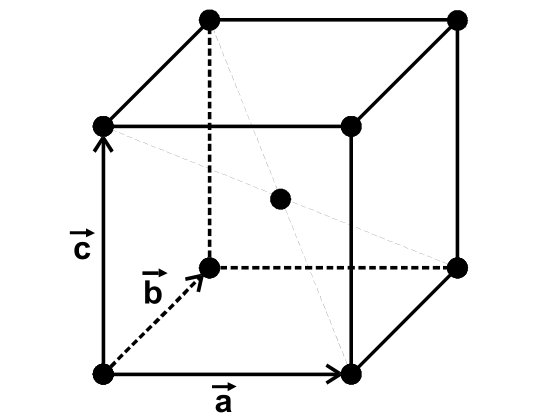
\includegraphics[width=\textwidth]{Abbildungen/raumzentriert}
		\subcaption{Das kubisch-raumzentrierte Gitter hat 2 Atome an den Orten (0,0,0) und $\left(\frac{1}{2}, \frac{1}{2}, \frac{1}{2} \right)$ und 8 nächste Nachbarn im Abstand von $\frac{1}{2}\sqrt{3}$a.}
	\end{minipage}
	\begin{minipage}[t]{0.45\textwidth}
		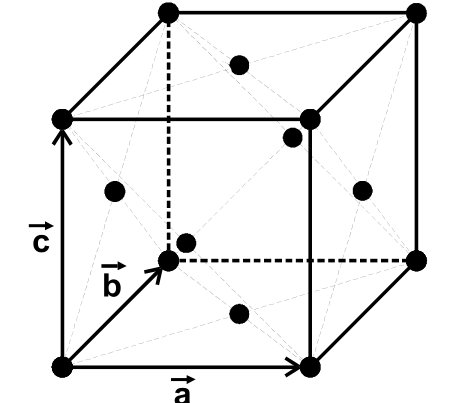
\includegraphics[width=\textwidth]{Abbildungen/flaechenzentriert}
		\subcaption{Das kubisch-flächenzentrierte Gitter hat 4 Atome an den Orten (0,0,0), $\left(\frac{1}{2}, \frac{1}{2}, 0 \right)$, $\left(\frac{1}{2}, 0, \frac{1}{2} \right)$, $\left(0, \frac{1}{2}, \frac{1}{2} \right)$  und besitzt 12 nächste Nachbarn im Abstand von $\frac{1}{2}\sqrt{2}$a.   }
\end{minipage}
\caption{Die Elementaren kubischen Gittertypen bei denen gilt $|a|=|b|= |c|$. \cite{Anleitung}}
\label{fig:gittertypen}
\end{figure}

In der Natur kristallieren Metalle und Salze nicht in einer so simplen kubischen Struktur. 
Die häufigste Struktur ist die Diamantstruktur. 
Sie besteht aus  zwei kubisch-flächenzentrierten Gittern die um ein viertel der Raumdiagonalen zueinander vorschoben sind. 
Es folgt, dass die Diamantstruktur acht Atome an den Orten
\begin{equation}
(0,0,0), \left(\frac{1}{2}, \frac{1}{2}, 0 \right), \left(\frac{1}{2}, 0, \frac{1}{2} \right), \left(0, \frac{1}{2}, \frac{1}{2} \right), \left(\frac{1}{4}, \frac{1}{4}, \frac{1}{4} \right), \left(\frac{3}{4}, \frac{3}{4}, \frac{1}{4} \right), \left(\frac{3}{4}, \frac{1}{4}, \frac{3}{4} \right),  \left(\frac{1}{4}, \frac{3}{4}, \frac{3}{4} \right)
\end{equation}
in der Einheitszelle aufweist.
Die vier nächsten Nachbarn jedes Atoms liegen auf einer Tetraeder Struktur um das Atom herum.
Dies entspricht der sp$^3$-Hybridiesierung des Kohlenstoffs und ist auch in Silizium und Germanium zu finden.\\
Die Diamantstruktur unterscheidet sich von der Zinkblende nur dadurch, dass die Zinkblende aus zwei unterschiedlichen Atomen besteht, die getrennt auf die jeweiligen fcc-Strukturen verteilt sind.\\
Salze kristallieren dahhingegen vielfältiger.
Es werden drei Arten vorgestellt.\\
Die erste ist die Steinsalz-Struktur. 
Sie ist wie die Diamantstruktur, wobei die fcc-Gitter diesmal um eine halbe Raumdiagonale gegneinander verschoben sind\\
Im Gegensatz dazu besteht die Casiumchlorid-Struktur aus zwei primitiven Gittern, die um eine halbe Raumdiagonale gegeneinander verschoben sind. 
Es entspricht der bcc-Struktur, wobei das Atom in der Mitte des Würfels nun ungleich dem am Rand ist.\\
Zuletzt wird noch die Fluorit-Struktur beschrieben.
Sie besteht aus drei fcc-Gittern, die jeweils um eine viertel Raumdiagonal gegeneinander verschoben sind. 
Das heißt, dass die Einheitszelle 12 Atome besitzt.\\\\
Die am dichtesten gepackte Kugelpackung, bei der gerade noch so Platz für alle Atome ist, ist in hexagonalen Gittern zu finden. 
Grundlage der hexagonalen Struktur, wie in Abbildung \ref{fig:hexagonal} zu sehen ist bilden die Raute mit $120\circ$  Winkeln.
\begin{figure}[h]
	\centering
	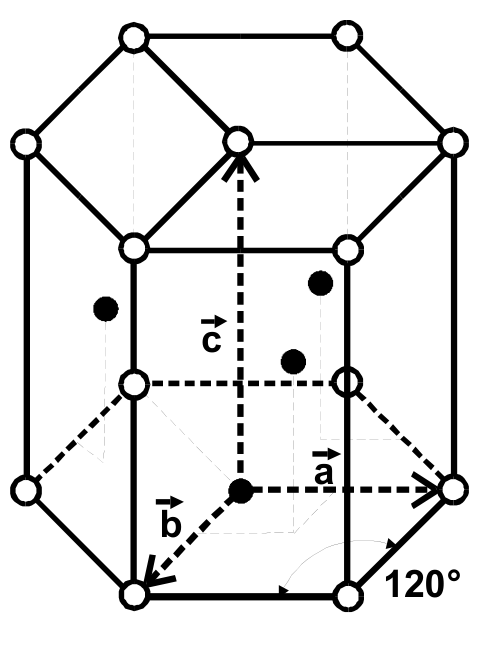
\includegraphics[width = 0.3\textwidth]{Abbildungen/hexagonal.png}
	\caption{Hexagonale Einheitszelle mit den Basisvektoren \cite{Anleitung}. }
	\label{fig:hexagonal}
\end{figure} 
Charakteristisch für die dichteste Kugelpackung ist das Achsenverhätnis von c/a = $\sqrt{\frac{8}{3}}$ wobei der Betrag der Basisvektoren $\vec{a}$ und $\vec{b}$ gleich sind.

\subsection{Millersche Indizes und Netzebenenabstand}
Wenn in einer Ebene die Schwerpunkte von Atomen eines Gitters liegen, so ist diese Ebene eine Netzebene.
Die millerschen Indizes werden durch die Netzebenen aufgestellt. 
Sie sind durch die Form (hkl) charakterisiert, wobei jede Zahl der Reziprokwert der Zahl ist, bei der die Netzebene eine der Achsen schneidet. 
Dies wird in Abbildung \ref{fig:miller} durch die beispielhafte Netzeben deutlich.

\begin{figure}[h]
	\begin{minipage}[t]{0.45\textwidth}
		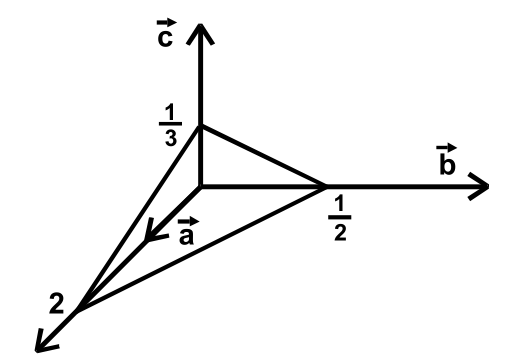
\includegraphics[width=\textwidth]{Abbildungen/miller}
		\subcaption{Netzebene mit den Millerindizes (146)}
	\end{minipage}
	\begin{minipage}[t]{0.45\textwidth}
		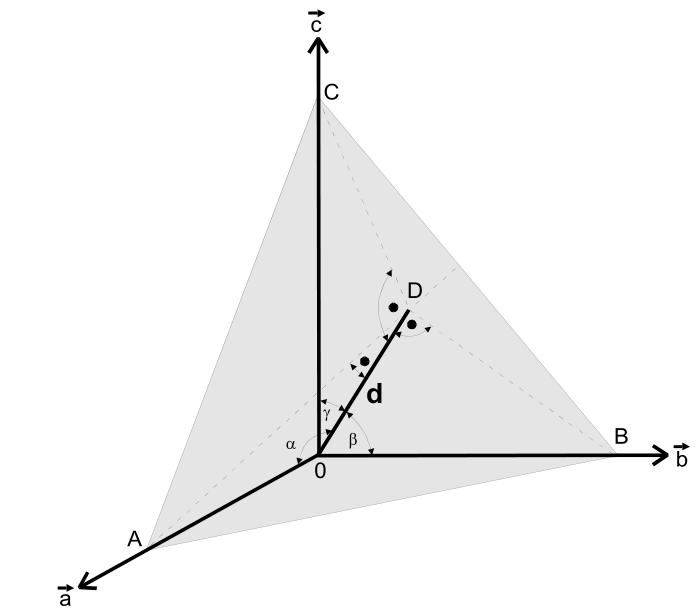
\includegraphics[width=\textwidth]{Abbildungen/netzebene}
		\subcaption{Schematische Darstellung des Netzebenenabstands d einer belibig gewählten Netzebene}
	\end{minipage}
	\caption{Beispielhafte Netzebenen zur Bestimmung der Millerindizes und des Netzebenenabstandes \cite{Anleitung}. }
	\label{fig:miller}
\end{figure}

Tritt der Fall auf, dass eine Netzeben im euklidischen Raum nur eine Achse schneidet, und die anderen beiden nicht, also der Wert $\infty$ ist, so ist der reziproke Wert 0. 
Beispiel für diesen Fall sind die Würfeloberflächen eines kubischen Gitters. 
Die obere Seite hat die Millerindizes (001).\\\\
Der Abstand einer Ebene zum Ursprung des Koordinatensystems wird durch den Netzebenenabstand d angegeben.
Der Netzebenanbstand ist der Betrag des Vektors $\vec{d}$, der stets senkrecht auf der Ebene steht und den Null-Punkt des Koordinatensystems mit dem der Ebene verbindet, wie in Abbildung \ref{fig:miller} gezeigt.
Alle höheren Netzebenen, die parallel zur ersten sind, haben genau den Abstand d voneinander.
Der Netzebenenabstand berechent sich wie folgt.
Die Dreiecke ODA, ODB, ODC in \ref{fig:miller} stehen senkrecht zueinander. Daraus folgt, dass
\begin{equation}
\cos{\alpha} = \frac{\text{d}\text{h}}{\text{a}}, \cos{\beta} = \frac{\text{d}\text{k}}{\text{b}}, \cos{\gamma} = \frac{\text{d}\text{l}}{\text{c}}
\label{eq:Abstand1}
\end{equation}
 und es gilt zusätzlich
\begin{equation}
\cos{\alpha}^2+\cos{\beta}^2+\cos{\gamma}^2 = 1
\label{eq:Abstand2}
\end{equation}
Werden nun die Gleichungen \ref{eq:Abstand1} und \ref{eq:Abstand2} ineinander eingesetzt, so ergibt sich für den Netzebenenabstand Gleichung \ref{eq:Abstand3}
\begin{equation}
\text{d} = \frac{1}{\sqrt{\frac{\text{h}}{\text{a}}^2+\frac{\text{k}}{\text{b}}^2+\frac{\text{l}}{\text{c}}^2}}
\label{eq:Abstand3}
\end{equation}
Ist das System kubisch, so gilt a = b = c und Gleichung (\ref{eq:Abstand4}).
\begin{equation}
\text{d} = \frac{\text{a}}{\sqrt{\text{h}^2+\text{k}^2+\text{l}^2}}
\label{eq:Abstand4}
\end{equation}

\subsection{Röntegnbeugung an Kristallen}
Röntgenstrahlen sind hochenergetische elektromagnetische Wellen, deren Wellenlänge im Bereich Angström liegt. 
Beim Eintritt in einen Kristall treten sie mit den Atomen in Wechselwirkung und werden im klassischen Sinne gestreut.
Die geladenen Teilchen q mit Masse m, an denen die Röntegstarhlung gestreut werden absorbieren die Energie und fangen selbst im Gittersystem an zu schwingen wie ein Hertzscher Dipol.
Die Intensität der abgegeben Strahlung ist in Gleichung (\ref{eq:dipol}) gegeben, wobei die Streuung an Atomkernen auf Grund ihrer hohen Masse zu vernachlässigen ist.
\begin{equation}
\text{I}_e(r,\theta) = \text{I}_0\times \left(\frac{\mu_0 \text{q}^2}{4 \pi \text{m}}\right) \frac{1}{r^2} \frac{1+\cos{2\theta}^2}{2}
\label{eq:dipol}
\end{equation}
Da nicht nur an einem Elektron gestreut wird, sondern an allen Netzebenen, gibt es Interfernezeffekte, die die Streuamplituden verstärken oder vernichten.
Diese Interfenzmuster sind abhängig vom Kristall, sodass aus dem Interfernzbild rückwirkend auf die Kristallstruktur geschlossen werden kann.
Die Wellenlänge der Röntgenstrahlung ca. genauso groß wie die Ausdehung der Atomhülle, sodass das atomare Streuvermögen nicht proportional zur Ordnungszahl z ist.
Die Gleichung (\ref{eq:dipol}) ist noch weiter zu modifizieren.
Denn die abgestrahlte Intensität von Elektronen, die später von dem Röntgenstrahl erfasst werden ist nicht so hoch wie die vorherige und es entsteht eine Phasendifferenz.
Das Verhältnis der gestreuten Intensität I$_e$ der Elektronen und I$_a$ der Atome ist das Quadrat des Atomformfaktors f und ist in Gleichung (\ref{eq:Aform}) dargestellt.
\begin{equation}
\text{f}^2 = \frac{\text{I}_a}{\text{I}_e}
\label{eq:Aform}
\end{equation}
Der Atomfomtfaktor ist abhängig von z, der Röntgenwellenlänge $\lambda$ und dem Streuwinkel $\theta$. 
Ist $\theta$ klein und $\lambda$ groß, so ist f $\approx$ z.
Die genau Bestimmung von f benötigt die Elektronendichteverteilung des Kristalls $\rho(\vec{\text{r}})$ über dessen Hülle phasenrichtig integriert werden muss.\\
Für die Bestimmung des Gangunterschieds einer einlaufenden und gestreuten EM-Welle wird die Skizze aus Abbildung (\ref{fig:streuung}) verwendet.
\begin{figure}[h]
	\begin{minipage}[t]{0.45\textwidth}
		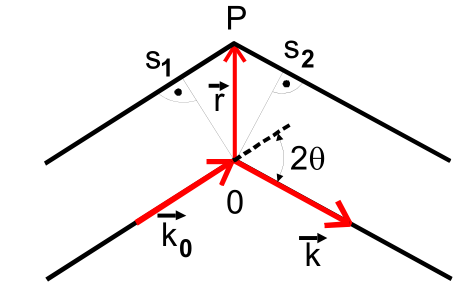
\includegraphics[width = \textwidth]{Abbildungen/streuung}
		\subcaption{Skizze, welche den Gangunterschied bei einem Streuprozess an zwei Punkten O und P zeigt.}
	\end{minipage}
	\begin{minipage}[t]{0.45\textwidth}
		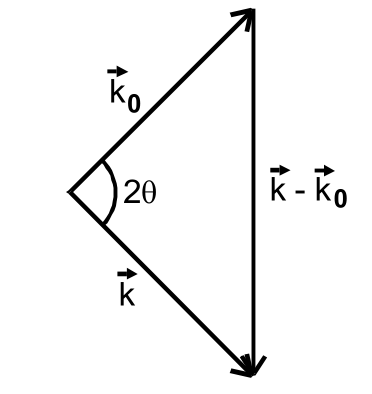
\includegraphics[width = \textwidth]{Abbildungen/streuwinkel}	
		\subcaption{Zusammenhang zwischen Streuwinkel und Wellenvektoren}
	\end{minipage}
	\caption{ Skizzierungen des Gangunterschieds $\Delta$s und der Streurichtung $\theta$ \cite{Anleitung}. }
	\label{fig:streuung}
\end{figure}
Zu beachten ist dabei, dass der Betrag der Wellenzahl der einlaufenden und der auslaufenden Welle gleich sind, wenn elsatische Streuung zu Grunde gelegt wird. Dann folgt Gleichung (\ref{eq:lambda}).
\begin{equation}
|\vec{\text{k}_0}| = |\vec{\text{k}}| = \frac{1}{\lambda}
\label{eq:lambda}
\end{equation} 
Der daraus resultierende Gangunterschied $\Delta $s aus Gleichung (\ref{eq:gangu}) lässt sich dann in die Phasendifferenz $\Delta \phi$ aus Gleichung (\ref{eq:phase}) überführen.
\begin{equation}
\Delta \text{s} = \text{s}_1+\text{s}_2 = \vec{\text{r}} \left( \frac{\vec{\text{k}}}{\text{k}} - \frac{\vec{\text{k}_0}}{k_0}  \right)
\label{eq:gangu} 
\end{equation}
\begin{equation}
\Delta \phi = 2\pi\frac{\Delta \text{s}}{\lambda} = 2\pi \vec{\text{r}} (\vec{\text{k}}-\vec{\text{k}_0})
\label{eq:phase} 
\end{equation}

Für die weitere Berechnung von f soll die Normierungsbedingung aus Gleichung (\ref{eq:normo}) gelten.
\begin{equation}
 \int_{\text{Hülle}} \rho (\vec{\text{r}}) \text{d}\text{r}^3 = \text{z}\text{e}_0
\label{eq:normo}
\end{equation}
Im Prinzip ist f eine Fouriertransformierte bezüglich der Ladungsdichteverteilung $\rho$, wie in Gleichung (\ref{eq:fourier}) zu erkennen ist,
\begin{equation}
\text{f} = \int_{\text{Hülle}} \text{e}^{-i\Delta\phi}\rho(\vec{\text{r}}) \text{d}\text{r}^3 = \int_{\text{Hülle}} \text{e}^{-i2\pi \vec{\text{r}}(\vec{\text{k}}-\vec{\text{k}_0})}\rho(\vec{\text{r}}) \text{d}\text{r}^3
\label{eq:fourier}
\end{equation}
wobei aus Abbildung (\ref{fig:streuung}) zu entnehmen ist, dass f abhängig von $\theta$ und $\lambda$ ist.
Veranschaulicht wird dies in Gleichung (\ref{eq:winkel})
\begin{equation}
|\vec{\text{k}}-\vec{\text{k}_0}| = \frac{2 \sin(\theta)}{\lambda}.
\label{eq:winkel}
\end{equation}
Damit ist die gestreute Intensität der Röntgenstrahlung an einem Atom abhängig vom Formfaktor f proportional zur Streuintensität I$_e$.\\\\
Die Streuung an einem Atom ist damit hinreichend diskutiert und muss nun auf die Streuung an einer Elementarzelle ausgeweitet werden.
Das Prinzip  einer Streuung zweier Wellen an zwei Atomen ist dabei analog zu dem vorherigen Prinzip.
Es ergibt sich wieder eine Phasendifferenz $\Delta \phi$ und eine daraus resultierende Streuamplitude aus Gleichung (\ref{eq:streuA}), die INterfenzefffekten unterlegen ist.
Dabei wird angenommen, dass ein Atom im Ursprung des Koordinatensystems liegt und die anderen im Abstand $\vec{\text{r}_j}$ folgen.
\begin{equation}
\text{A} = \sum_j \text{f}_j \text{e}^{-2\pi i \vec{\text{r}_j} (\vec{\text{k}}-\vec{\text{k}_0}) } \text{I}_e
\label{eq:streuA}
\end{equation}
Da die $\vec{\text{r}_j}$ gerade Atome auf dem Gitter sind, ist der Vektor durch die Basisvektoren darzustellen.
Wird dies ausgenutzt, so egibt sich die Strukturamplitude (\ref{eq:Struk}) der Elementarzelle.
\begin{equation}
\text{S} = \sum_j \text{f}_j \text{e}^{-2\pi i (x\vec{\text{a}}+y \vec{\text{b}}+ z \vec{\text{c}}) (\vec{\text{k}}-\vec{\text{k}_0}) } \text{I}_e
\label{eq:Struk}
\end{equation}
Nun ist noch zu beachten, dass nicht nur an zwei Atomen einer Elementarzelle, sondern an der gesamten Elementarzelle gestreut wird. 
Unter der Berücksichtigung des Huygenschen Prinzips, dass die ein und auslaufenden Wellen nur dann einen Reflex ergeben, wenn sie symmetrisch zur Netzebenennormalen liegen, ergeben sich erhebliche Einschränkungen für die sichtbaren Reflexe.
Denn Reflex ist erst dann sichtbar, wenn er durch positive Interferent verstärkt wird. Denn der Beugungsreflex eines einzelnen Atoms ist viel zu schwach.
Da aber der Röntgenstrahl an mindestens 10$^3$ Netzebenen gestreut wird, wird ein Signal durch positive Interferenz sichtbar.
Wie eine Struung an einer Netzebenenschar aussehen kann ist beispielhaft in Abbildung (\ref{fig:bragg}) gezeigt.
\begin{figure}[h]
	\centering
	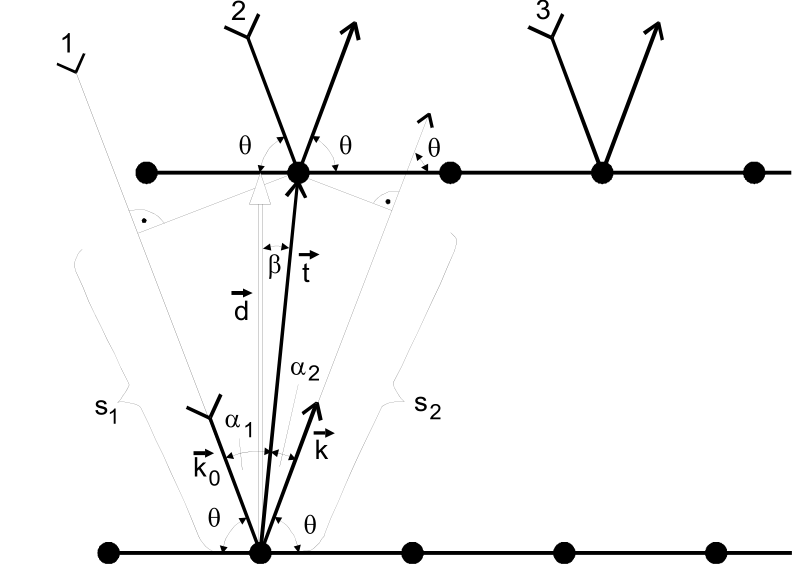
\includegraphics[width = 0.5\textwidth]{Abbildungen/bragg}
	\caption{Schematisch Struktur eines Reflexes, der der Bragg-Bedingung unterliegt}
	\label{fig:bragg}
\end{figure}
Aus der Skizze folgt für den Gangunterschied in (\ref{eq:gang2}) 
\begin{equation}
\text{n} \lambda = \Delta \text{s}_1+\Delta \text{s}_2 = \text{t}(\cos{\alpha_1}+cos{\alpha_2})
\label{eq:gang2}
\end{equation}
und daraus ergibt sich dann die Bragg-Bedingung aus Gleichung (\ref{eq:bragg}).
\begin{equation}
\text{n}\lambda = 2 \text{d} \sin{\theta}
\label{eq:bragg}
\end{equation}
Dabei ist d der Netzebenenabstand und n Element der natürlichen Zahlen $\mathbb{N}$.
Mit Hilfe von reziproken Vektoren, die senkrecht auf der Netzebene stehen und den Betrag n/$|\vec{\text{d}}|$ stellt sich die Braggbedingung wie folgt dar
\begin{equation}
 \text{n} = \vec{ \text{d}}(\vec{ \text{k}}-\vec{ \text{k}_0}).
\end{equation}
Daraus folgt dann die modifizierte Strukturamplitude in Gleichung (\ref{eq:Struk2})
\begin{equation}
\text{S}(hkl) = \sum_j \text{f}_j \text{e}^{-2\pi i (x\vec{\text{a}}+y \vec{\text{b}}+ z \vec{\text{c}}) (\vec{\text{k}}-\vec{\text{k}_0})\times (h\vec{\text{A}}+k\vec{\text{B}}+ l\vec{\text{C}}) } = \sum_j \text{f}_j \text{e}^{-2\pi i (xh+y k+ z l) }
\label{eq:Struk2}
\end{equation}
Die Großbuchstaben sind dabei die reziproken Gittervektoren zu den Basisvektoren.
\begin{equation}
s
\label{eq:g}
\end{equation}
\newpage
\section{Durchführung}
\label{sec:Durchführung}
\subsection{Versuchsaufbau}
Zentral in diesem Versuch ist die Röntgenstrahlung welche durch eine Öffnung an der Mantelfläche eines Zylinders, in dessen Mitte das Probenstäbchen sitzt, auf die Probe gestrahlt wird und dabei gestreut wird. 
Die Innenseite des Mantels des Metallzylinders ist vollständig mit einem Film bedeckt.
Die Achse des Probenstäbchens steht senkrecht auf den beiden Deckeln des Zylinders. Eine schematische Skizze das Aufbaus ist in \ref{fig:Aufbau} gegeben.
\begin{figure}
	\centering
	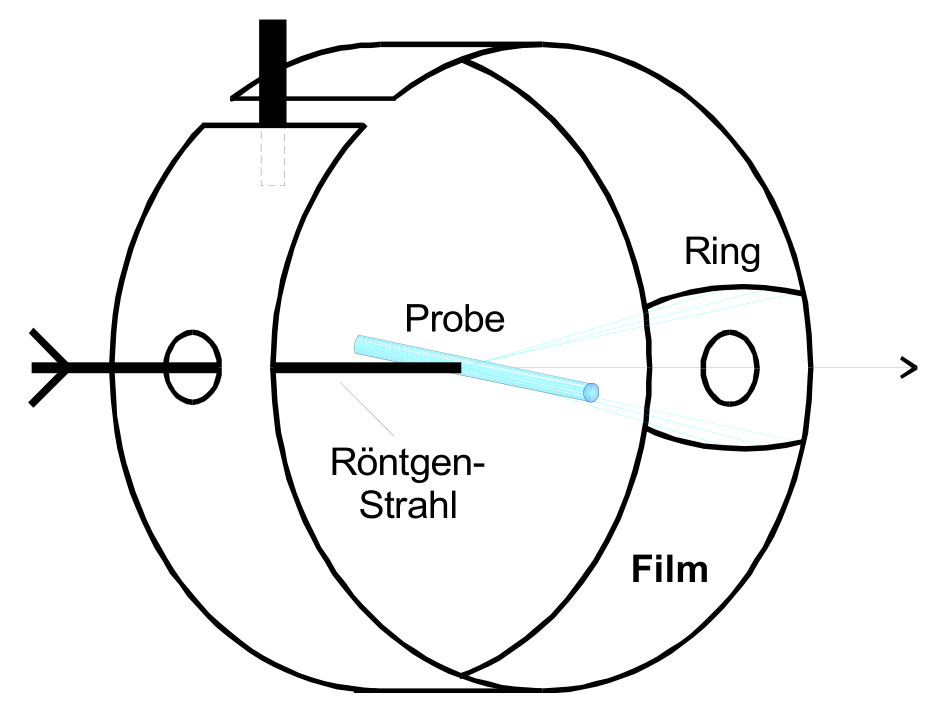
\includegraphics[width = 0.5\textwidth]{Abbildungen/Aufbau.png}
	\caption{Der Aufbau zeigt den Film in der Kamera, sowie die Probe und den EIngang der Röntgenstrahlung und ein mögliches Beugungsmuster an der rechten Seite des Films in der Skizze \cite{Anleitung}. }
	\label{fig:Aufbau}
\end{figure}  
Der ganze Zylinder ist bis auf die Öffnung für die Röntgenstrahlung lichtdicht verschlossen.
Außen am Zylinder, an der Fassung des Probenstäbchens ist ein Motor angebracht, mit dem die Probe gedreht wird.
Der Zylinder ist sozusagen das Kameragehäuse und wird im weiteren Verlauf als Kamera bezeichnet. 
Die Fassung selber ist so justierbar, dass das Probenstäbchens möglichst mittig zur Öffnung des Röngenstrahls steht.\\
Die Röntgenstrahlen werden durch eine Röntgenröhre erzeugt, welche eine Kupferanode besitzt.
Die Beschleunigungsspannung ist dabei deutlich gräßer, als die Kathodenspannung und beträgt \SI{40}{\kV}. 
Dabei werden die charakterisctischen Emissionslinien K$_{\alpha 1}$, K$_{\alpha 2}$ und K$_\beta$ erzeugt. 
Die K$_\beta$-Linie ist ncht relevant.  
Sie wird durch Nickel absorbiert.

\subsection{Preparation der Probe}
Das Probenstäbchen ist ein einfaches Glasstäbchen, welches mit dem zu untersuchenden Stoff benetzt wird.
Dazu wird das Probenstäbchen in Vaseline eingetacht und dann in dem Probenmaterial gedreht, sodass eine dünne Schicht auf der Oberfläche des Stäbchens entsteht. 
Die Stäbchen messen alle ungefähr 0.8 \si{\milli \meter} im Durchmesser.
Dann muss das präparierte Probenstäbchen in einen passenden Halter gesteckt und dann in die Kamera eingebaut werden.

\subsection{Entwicklung der Filme}
Der Film wird dann in einer Dunkelkammer entwickelt. 
Das wird in drei Stufen ausgeführt, wobei zwischen den drei Phasen der Film in einem Wasserbad durch Schwenken gereiningt wird.\\
In der ersten Phase wird der Film auf eine Spule gewickelt und in ein Gefäß mit Entwicklungsflüssigkeit 15 Minuten lang geschwenkt.
Die zweite Phase nutzt einen UNterbrecherbad, in der der Film ca. 1 Minute lang getacht wird. \\
Zum Schluss wird der Film dann wieder, in einem Gefäß mit einer Fixierflüssigkeit, 5 Minuten lang geschwenkt.
Danach trocknet der Film 30 Minuten in einer Heißluftkammer.
 








\newpage
\section{Auswertung}
\label{sec:Auswertung}

Nach der Messung werden die Filmstreifen ausgemessen. Dies geschieht aufgrund von fehlenden Werkzeugen mit einem gemeinen Lineal. Der systematische Fehler wird dabei auf $\pm\SI{1}{mm}$ gesetzt. Gemessen wird der Abstand zwischen zwei Linien, also der Kegelradius. Der Abstand zwischen dem Eintritts- und dem Austrittsloch beträgt \SI{180}{mm} und deckt einen Winkel $\pi$ der Kammer ab. Wie in Abbildung \ref{fig:sys2} zu sehen ist, wird in einer Hälfte der Kammer zwischen Eintritts- und Austrittsloch ein Winkel von $2\theta$ abgedeckt. Daraus lässt sich $\theta$ mit Gleichung (\ref{eqn:theta}) berechnen.
\begin{equation}
\label{eqn:theta}
	2\theta = x \cdot \frac{\pi}{\SI{180}{mm}} \Longrightarrow \theta = x \cdot \frac{\pi}{\SI{360}{mm}}
\end{equation}
Hierbei ist $x$ der Kegelradius. In Tabelle \ref{tab:KegelMetall} sind die gemessenen Kegelradien und die zugehörigen Winkel für Metall zu sehen. In Tabelle \ref{tab:KegelSalz} entsprechendes für Salz.
%
% \begin{table}[h]
% \centering
% \caption{Kegelradien gemessen an den Filmstreifen umgerechnet in den Winkel $\theta$ für Metall.}
% \label{tab:Kegel}
% 	\begin{minipage}[t]{0.4\textwidth}
% 	% \begin{table}[h]
% 	% \centering
% 	\caption{}
% 	\label{tab:KegelMetall}
% 	\begin{tabular}{c | c}
% 			\hline
% 			\text{Kegelradius $x$ [mm]} & \text{Winkel $\theta$} \\
% 			\hline
% 			44.5\pm1 &  0.388\pm0.009 \\
% 			64.5\pm1 &  0.563\pm0.009 \\
% 			81.5\pm1 &  0.711\pm0.009 \\
% 			98.5\pm1 &  0.860\pm0.009 \\
% 			114.5\pm1 & 0.999\pm0.009 \\
% 			134.5\pm1 & 1.174\pm0.009 \\
% 			\hline
% 	\end{tabular}
% 	% \end{table}
% 	\end{minipage}
% 	%
% 	\begin{minipage}[t]{0.4\textwidth}
% 	% \begin{table}[h]
% 	% \centering
% 	\caption{}
% 	\label{tab:KegelSalz}
% 	\begin{tabular}{c | c}
% 			\hline
% 			\text{Kegelradius $x$ [mm]} & \text{Winkel $\theta$} \\
% 			\hline
% 			23\pm1 & 0.240\pm0.009 \\
% 			34.5\pm1 & 0.340\pm0.009 \\
% 			43\pm1 & 0.415\pm0.009 \\
% 			51\pm1 & 0.484\pm0.009 \\
% 			57\pm1 & 0.537\pm0.009 \\
% 			65\pm1 & 0.607\pm0.009 \\
% 			78\pm1 & 0.720\pm0.009 \\
% 			83\pm1 & 0.764\pm0.009 \\
% 			90\pm1 & 0.825\pm0.009 \\
% 			95.5\pm1 & 0.873\pm0.009 \\
% 			103\pm1 & 0.938\pm0.009 \\
% 			108\pm1 & 0.982\pm0.009 \\
% 			116\pm1 & 1.052\pm0.009 \\
% 			133\pm1 & 1.200\pm0.009 \\
% 			\hline
% 	\end{tabular}
% 	% \end{table}
% 	\end{minipage}
% \end{table}
%
\begin{table}[h]
\centering
\caption{Kegelradien gemessen an den Filmstreifen umgerechnet in den Winkel $\theta$ für Metall.}
\label{tab:KegelMetall}
\begin{tabular}{c | c}
		\hline
		\text{Kegelradius $x$ [mm]} & \text{Winkel $\theta$} \\
		\hline
		44.5\pm1 &  0.388\pm0.009 \\
		64.5\pm1 &  0.563\pm0.009 \\
		81.5\pm1 &  0.711\pm0.009 \\
		98.5\pm1 &  0.860\pm0.009 \\
		114.5\pm1 & 0.999\pm0.009 \\
		134.5\pm1 & 1.174\pm0.009 \\
		\hline
\end{tabular}
\end{table}
\begin{table}[h]
\centering
\caption{Kegelradien gemessen an den Filmstreifen umgerechnet in den Winkel $\theta$ für Salz.}
\label{tab:KegelSalz}
\begin{tabular}{c | c}
		\hline
		\text{Kegelradius $x$ [mm]} & \text{Winkel $\theta$} \\
		\hline
		27.5\pm1 & 0.240\pm0.009 \\
		39.0\pm1 & 0.340\pm0.009 \\
		47.5\pm1 & 0.415\pm0.009 \\
		55.5\pm1 & 0.484\pm0.009 \\
		61.5\pm1 & 0.537\pm0.009 \\
		69.5\pm1 & 0.607\pm0.009 \\
		82.5\pm1 & 0.720\pm0.009 \\
		87.5\pm1 & 0.764\pm0.009 \\
		94.5\pm1 & 0.825\pm0.009 \\
		100.0\pm1 & 0.873\pm0.009 \\
		107.5\pm1 & 0.938\pm0.009 \\
		112.5\pm1 & 0.982\pm0.009 \\
		120.5\pm1 & 1.052\pm0.009 \\
		137.5\pm1 & 1.200\pm0.009 \\
		\hline
\end{tabular}
\end{table}
Für spätere Berechnungen wird außerdem der Netzebenenabstand $d$ benötigt.
\begin{equation}
\label{eqn:d}
	d = \frac{\lambda}{2\sin(\theta)}
\end{equation}

\subsection{Nicht verschwindende Reflexe}

Mit den bestimmten Winkeln und Gleichung (\ref{eq:Struk2}) kann nun die Strukturamplitude für verschiedene Netzebenen und damit verschiedene $[hkl]$-Werte bestimmt werden. Genau genommen ist für die Bestimmung der nicht verschwindenden Reflexe nur interessant ob $S(hkl)$ verschwindet oder nicht. In Tabelle \ref{tab:Strukturen} sind für die kubischen Gitter (SC, BCC, FCC und Diamant) die ersten sechs, laut Theorie, nicht verschwindenden Reflexe.
%
\begin{table}[h]
\centering
\caption{Es sind für die kubischen Gitter (SC, BCC, FCC und Diamant) die ersten sechs, laut Theorie, nicht verschwindenden Reflexe dargestellt.}
\label{tab:Strukturen}
\begin{tabular}{c | c | c | c}
		\hline
		SC & BCC & FCC & Diamant \\
		\hline
		100 & 110 & 111 & 111 \\
		110 & 200 & 200 & 220 \\
		111 & 211 & 220 & 311 \\
		200 & 220 & 311 & 400 \\
		210 & 310 & 222 & 331 \\
		211 & 222 & 400 & 422 \\
		\hline
\end{tabular}
\end{table}

Für die Strukturbestimmung des Salzes (Zinkblende-, Steinsalz-, Caesiumchlorid- und Fluoritstruktur) müssen die Formfaktoren in Gleichung (\ref{eq:Struk2}) berücksichtigt werden. Deswegen kann nicht bestimmt werden ob die Reflexe verschwinden, sondern nur die Intensität der Linien.

\subsection{Bestimmung der Kristallstruktur}

Aus Gleichung (\ref{eq:Abstand4}) und (\ref{eqn:d}) folgt
\begin{equation*}
	d = \frac{a}{\sqrt{h^2 + k ^2 + l^2}} = \frac{a}{m} = \frac{\lambda}{2\sin(\theta)} \text{ mit }m\equiv\sqrt{h^2 + k ^2 + l^2}.
\end{equation*}
Damit lässt jedes $m$ auf den ersten nicht verschwindenden Reflex normieren und mit den experimentell bestimmten Werten vergleichen:
\begin{equation*}
	\frac{m_i}{m_1} = \frac{\sin{\theta_i}}{\sin{\theta_1}}.
\end{equation*}
Durch den Vergleich von Daten und Theorie wird die Struktur bestimmt. In Abbildung \ref{fig:verhaeltnisse} ist die Übereinstimmung der Verhältnisse jeweils für Metall und Salz zu sehen. Des weiteren wird die Abweichung der Daten von der Theorie bestimmt durch
\begin{equation*}
	\Chi^2 = \sum\frac{\left(\frac{\sin{\theta_i}}{\sin{\theta_1}} - \frac{m_i}{m_1}\right)^2}{\frac{m_i}{m_1}}.
\end{equation*}
Wie bereits in Abbildung \ref{fig:verhaeltnisse_metall} zu sehen ist, lässt sich das SC- und das BCC-Gitter für Metall mit so wenigen Daten nicht unterscheiden. Die Werte für alle Gitter sind in Tabelle \ref{tab:Xi} zu sehen.
%
\begin{table}[h]
\centering
\caption{Es sind für die kubischen Gitter (SC, BCC, FCC und Diamant) die $\Chi^2$ dargestellt.}
\label{tab:Xi}
\begin{tabular}{c | c | c | c | c}
		\hline
		& SC & BCC & FCC & Diamant \\
		\hline
		$\Chi^2$ & $0.0002\pm0.0018$ & $0.0002\pm0.0018$ & $0.10\pm0.04$ & $0.18\pm0.05$ \\
		\hline
\end{tabular}
\end{table}
%
\begin{figure}[h]
	\begin{minipage}[t]{0.45\textwidth}
		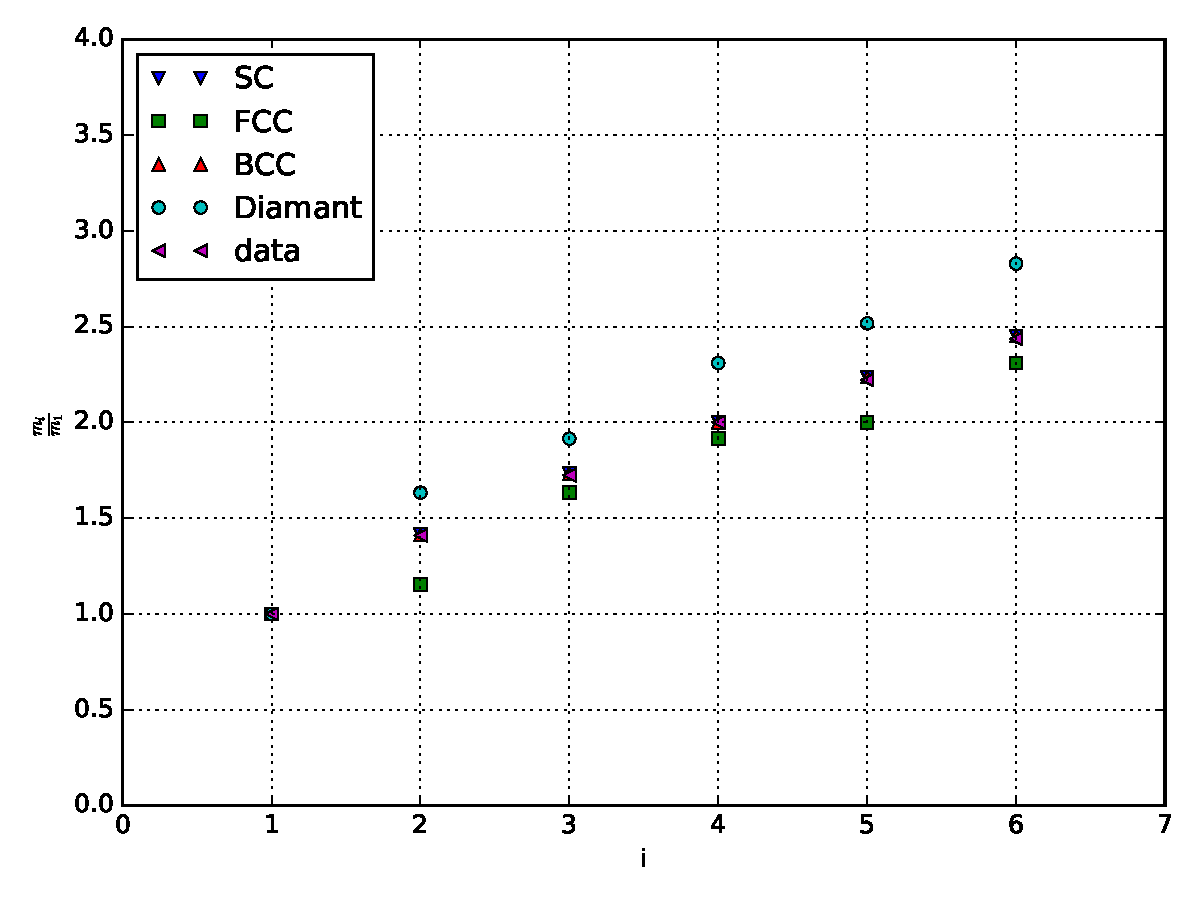
\includegraphics[width=\textwidth]{Abbildungen/verhaeltnisse.pdf}
		\subcaption{Verhältnisse $\frac{m_i}{m_1}$ für verschiedene Gittertypen und Daten für Metall.}
		\label{fig:verhaeltnisse_metall}
	\end{minipage}
	\begin{minipage}[t]{0.45\textwidth}
		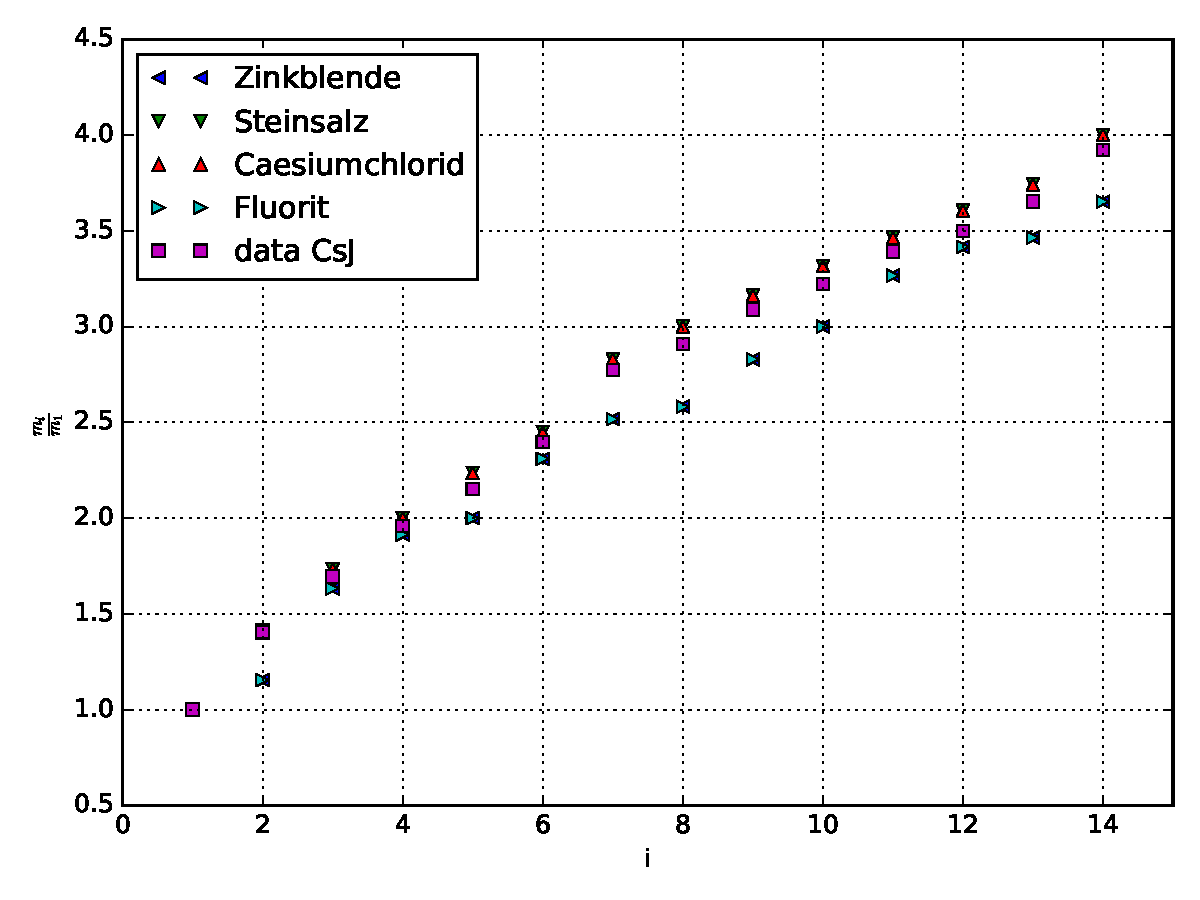
\includegraphics[width=\textwidth]{Abbildungen/verhaeltnisse_Salz.pdf}
		\subcaption{Verhältnisse $\frac{m_i}{m_1}$ für verschiedene Gittertypen und Daten für Salz.}
		\label{fig:verhaeltnisse_salz}
\end{minipage}
% \caption{Die Elementaren kubischen Gittertypen bei denen gilt $|a|=|b|= |c|$. \cite{Anleitung}}
\label{fig:verhaeltnisse}
\end{figure}
Da es nur drei Stoffe mit einer SC-Struktur gibt (Sauerstoff, Fluor und Polonium) ist bei dem Metall-Pulver von einer BCC-Struktur auszugehen. Für Salz wurde das gleiche Prozedere benutzt, nur dass diesmal die Formfaktoren, in Abbildung \ref{fig:formfaktoren} zu sehen, berücksichtigt werden müssen. Das bedeutet, dass für jede Struktur (Zinkblende-, Steinsalz-, Caesiumchlorid- und Fluoritstruktur) jede mögliche Kombination der Ionen, die in Abbildung \ref{fig:formfaktoren} zu sehen sind, getestet werden muss. Die theoretischen Verhältnisse $m_i / m_1$ geplottet gegen die Daten von Caesiumiodid (CsJ) sind in Abbildung \ref{fig:verhaeltnisse_salz} zu sehen. CsJ in der Caesiumchlorid-Sturktur ist der Stoff, der die kleinste Abweichung hat. 
% Die Abweichungen für jede Kombination sind in Tabelle \ref zu sehen.
\begin{figure}[h]
\centering
	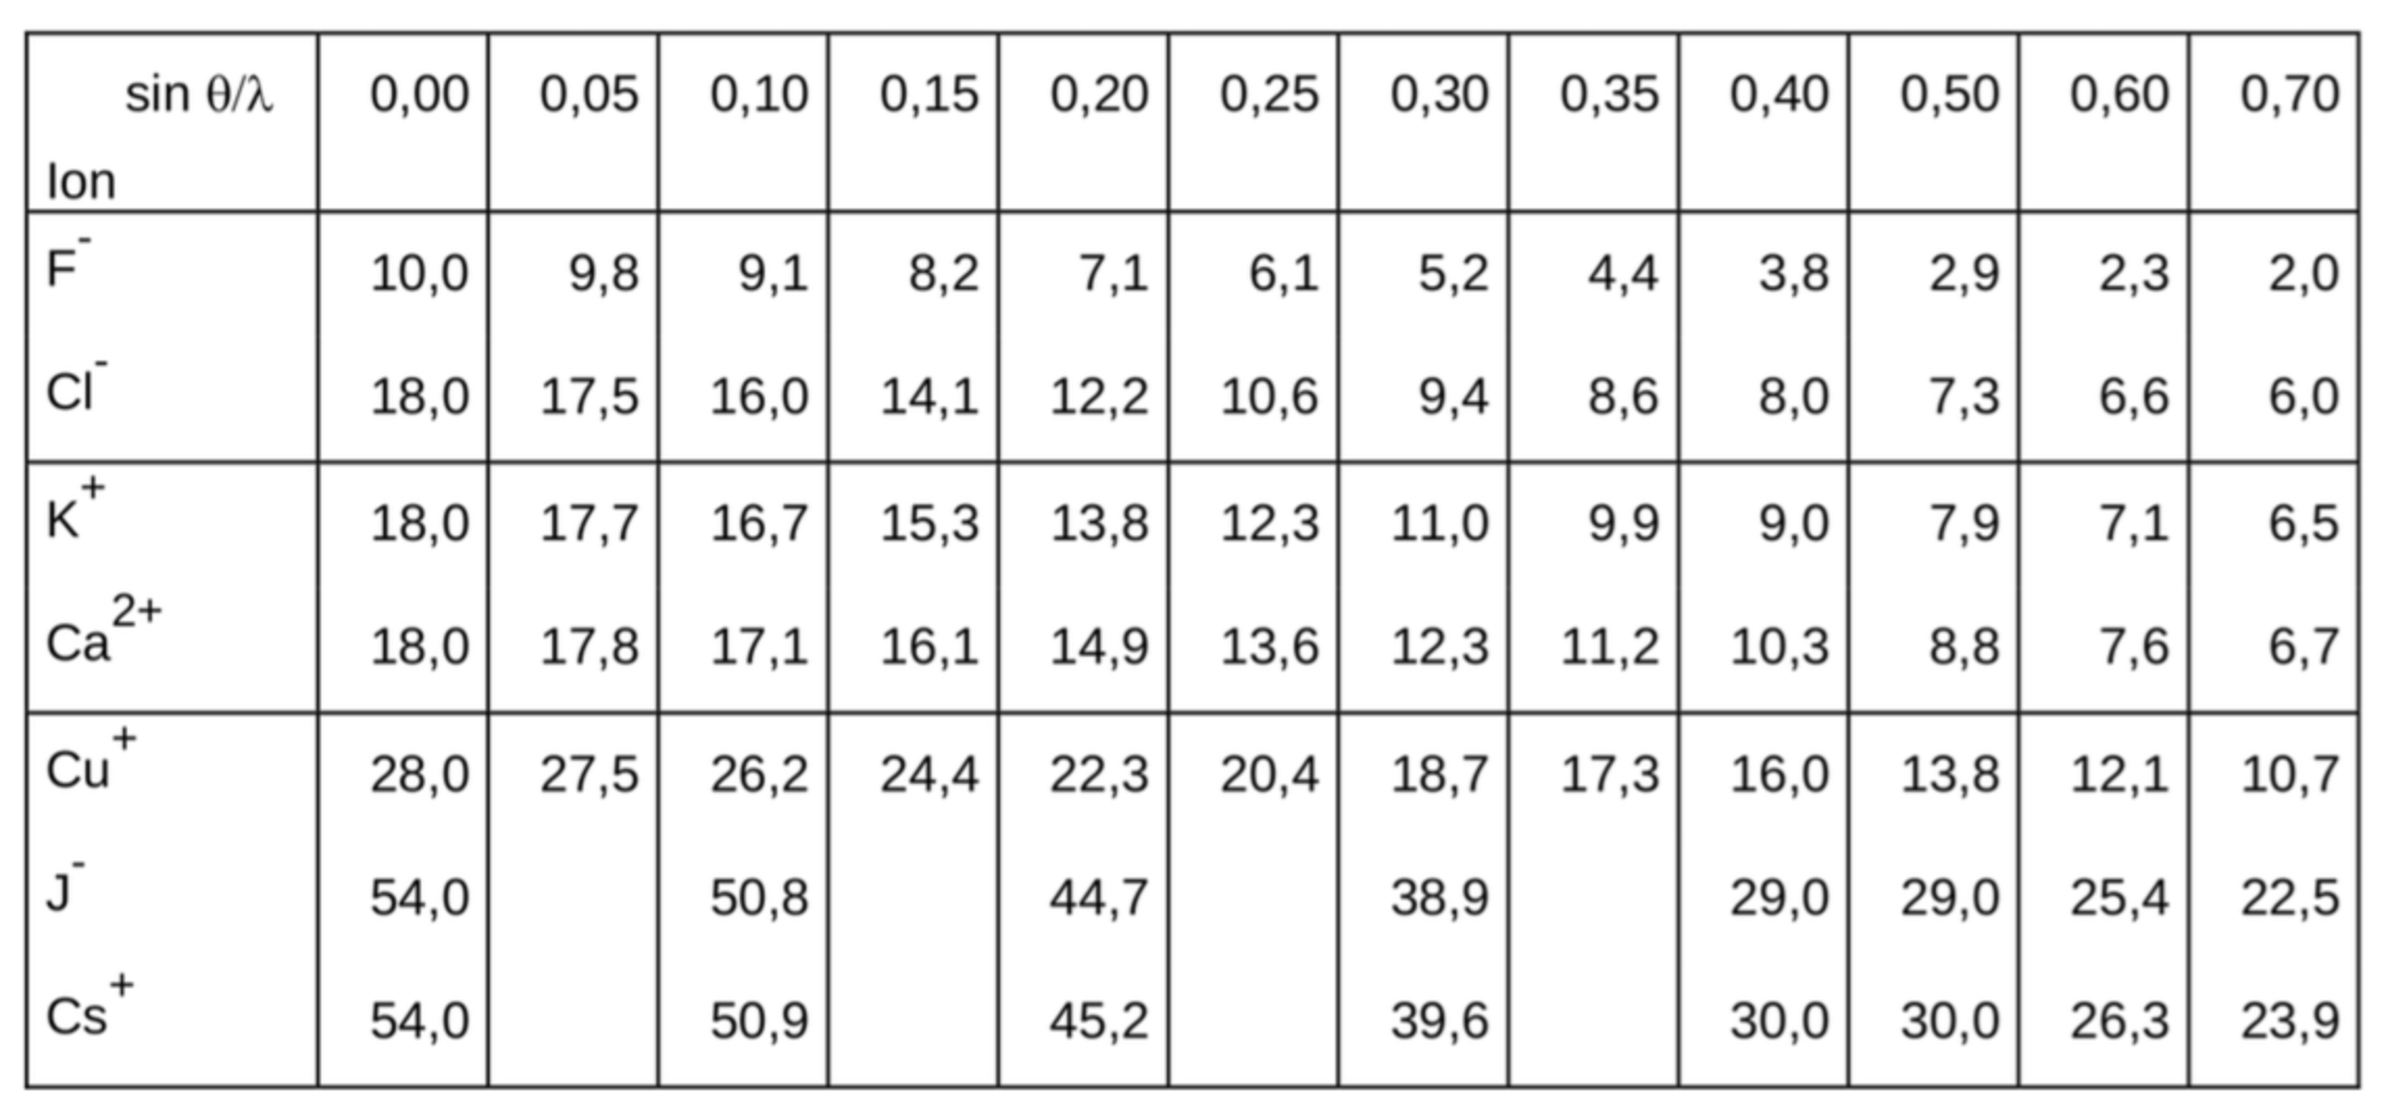
\includegraphics[width = 0.9\textwidth]{Abbildungen/formfaktoren.pdf}
\caption{Die Formfaktoren für verschiedene Ionen, je nach Winkel \cite{Anleitung}.}
\label{fig:formfaktoren}
\end{figure}

\subsection{Systematische Fehler}

Als Erstes ist darauf hinzuweisen, dass durch den Versuchsaufbau zwei systematische Fehler gemacht werden, die wie folgt in die Auswertung einfließen.
Die Systematischen Fehler entstehen bei den Ringradien. 
Dabei entsteht der Eindruck, dass die Gitterkonstante a abhängig von dem Beugungswinkel $\theta$ ist. \\
Der erste systematische Fehler liegt in der Messung von dem 4 $\theta$-Winkel, der stets zu groß gemessen wird. 
Problematisch ist das so kleine Winkel große Fehler besitzen. 
in Abbildung \ref{fig:sys1} wird schematisch gezeigt, wie das wahre $\theta$ aussehen sollte.
\begin{figure}
\centering
	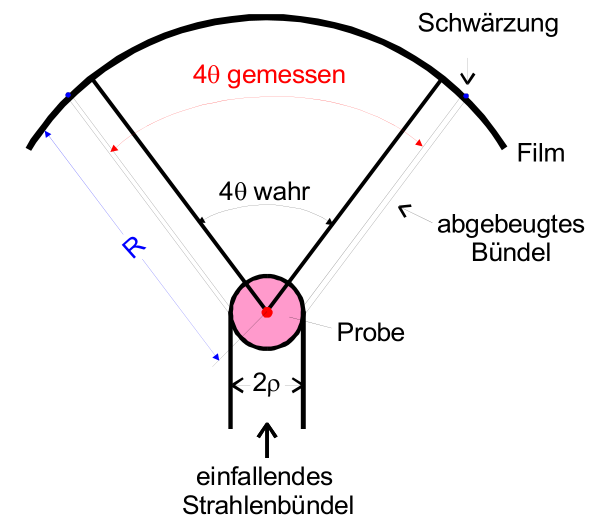
\includegraphics[width = 0.5\textwidth]{Abbildungen/Syst1.png}
	\caption{Darstellung des systematischen Fehlers, der aus der Absorbtion innerhalb des Probenstäbchens entsteht \cite{Anleitung}.}
	\label{fig:sys1}
\end{figure} 
Das Problem liegt darin, dass der Großteil der Strahlung komplett absorbiert wird und nur am Rand Beugungseffekte entstehen die aus der Probe kommen.
Berücksichtigt wird dies durch die Korrektur $\Delta a_A$ nach Bradley und Jay in Gleichung \ref{eq:syst1}.
\begin{equation}
\frac{\Delta a_A}{\text{a}} = \frac{\rho}{2\text{R}}\left( 1-\frac{\text{R}}{\text{F}} \right)\frac{\cos^2{\theta}}{\theta}
\label{eq:syst1}
\end{equation}
Der Größen sind in der Abbildung \ref{fig:sys1} dargestellt. 
$\rho$ ist der Radius des Probenstäbchens, R der Kameraradius und F der Abstand zwischen Fokus und Probe.
Dieser Fehler führt in dem Plot von $a(\theta)$ gegen $\cos^2{\theta}$ zu den Fehlerbalken in a.
\\\\
Der Zweite Systematische Fehler resultiert aus der Geometrie des Aufbaus.
In der Regel sind die Achse des Probenzylinders und die Achse des Films leicht gegeneinander verschoben. 
Das ist in Abbildung \ref{fig:sys2} dargestellt.
\begin{figure}
\centering
	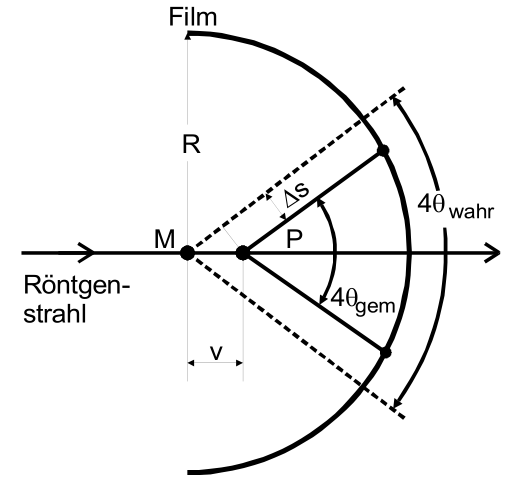
\includegraphics[width = 0.5\textwidth]{Abbildungen/Syst2.png}
	\caption{\cite{Anleitung}.}
	\label{fig:sys2}
\end{figure}
Dieser Fehler wirkt sich wieder auf das gemessene $\theta$ aus und ergibt die Abweichung $\Delta \theta$ wie in Gleichung \ref{eq:syst2} aufgeführt ist.
Der Abstand $\Delta$S und die Verschiebung v sind aus der Skizze \ref{fig:sys2} zu entnehmen.
\begin{align*}
\Delta \text{S} &  = -\text{v} \sin{2 \theta} \\
\Delta \theta & = -\frac{\Delta \text{S}}{2\text{R}}
\end{align*}
\begin{equation}
\Delta \theta = \frac{\text{v}}{2\text{R}}\sin{2\theta} = \frac{\text{v}}{\text{R}}\cos{\theta}\sin{\theta}
\label{eq:syst2}
\end{equation}
Unter Berücksichtigung der differnzierten Bragg-Bedingung ergibt sich der Korrekturterm $\Delta a_v$ in Gleichung \ref{eq:system} aus
\begin{align*}
\frac{\Delta \text{a}}{\text{a}} = \frac{\Delta \text{d}}{\text{d}} = -\Delta \theta \frac{\cos{\theta}}{\sin{\theta}}.
\end{align*}
\begin{equation}
\frac{\Delta a_v}{\text{a}} = \frac{\text{v}}{\text{R}}\cos^2{\theta}
\label{eq:system}
\end{equation}
Das heißt, die Gesamte Abweichung der Gitterkonstante resultiert in $\Delta a_{ges}$, welche as der Summe der beiden systematischen Fehler $\Delta a_A$ und $\Delta a_v$. 
Dabei ist die Gitterkonstante $\Delta a_{ges}$ proportional zu $\cos2{\theta}$.\\
Die tatsächliche Gitterkonstante a ist deshalb aus dem y-Achsenabschnitt des Plots $a(\theta)$ gegen $\cos^2{\theta}$ zu entnehmen.

<<<<<<< 3919e70f61e226b74a65735ba5c73a3a4af72710
\subsection{Metall}
||||||| merged common ancestors
ajwkhfkgWVUIwbefbbWJHEBFBHKJAEBKJFHWEHFVV
=======

\subsection{Metall}

ajwkhfkgWVUIwbefbbWJHEBFBHKJAEBKJFHWEHFVV
>>>>>>> Ein bisschen an der Auswertung getexet
=======
\subsection{Gitterkonstante}

Um den systematischen Fehler nach Gleichung (\ref{eq:system}) zu eliminieren und damit die Gitterkonstante zu bestimmen wird die Gitterkonstante $a$ gegen $\cos^2(\theta)$ geplottet und ein linearer Fit vollzogen. In Abbildung \ref{fig:fit_metall} ist der Fit für Metall zu sehen. In Abbildung \ref{fig:fit_salz} der Fit für Salz. Für Metall ergibt sich eine Gitterkonstante von $a_{metall} = \SI{2.86(18)e-10}{m}$, welche ziemlich genau mit dem Literaturwert von $a_{metall}^{lit} = \SI{2.86e-10}{m}$ \cite{metall} übereinstimmt. In Abbildung \ref{fig:fit_salz} ist der Fit für die Salz-Struktur zu sehen. Es wurde bereits durch die Strukturanalyse CsJ vorhergesagt. Der Fit liefert eine Gitterkonstante von $a_{salz} = \SI{4.48(20)e-10}{m}$ welche gut mit dem Literaturwert von $a_{salz}^{lit} = \SI{4.57e-10}{m}$ \cite{Gross} übereinstimmt.

\begin{figure}[h]
	\begin{minipage}[t]{0.45\textwidth}
		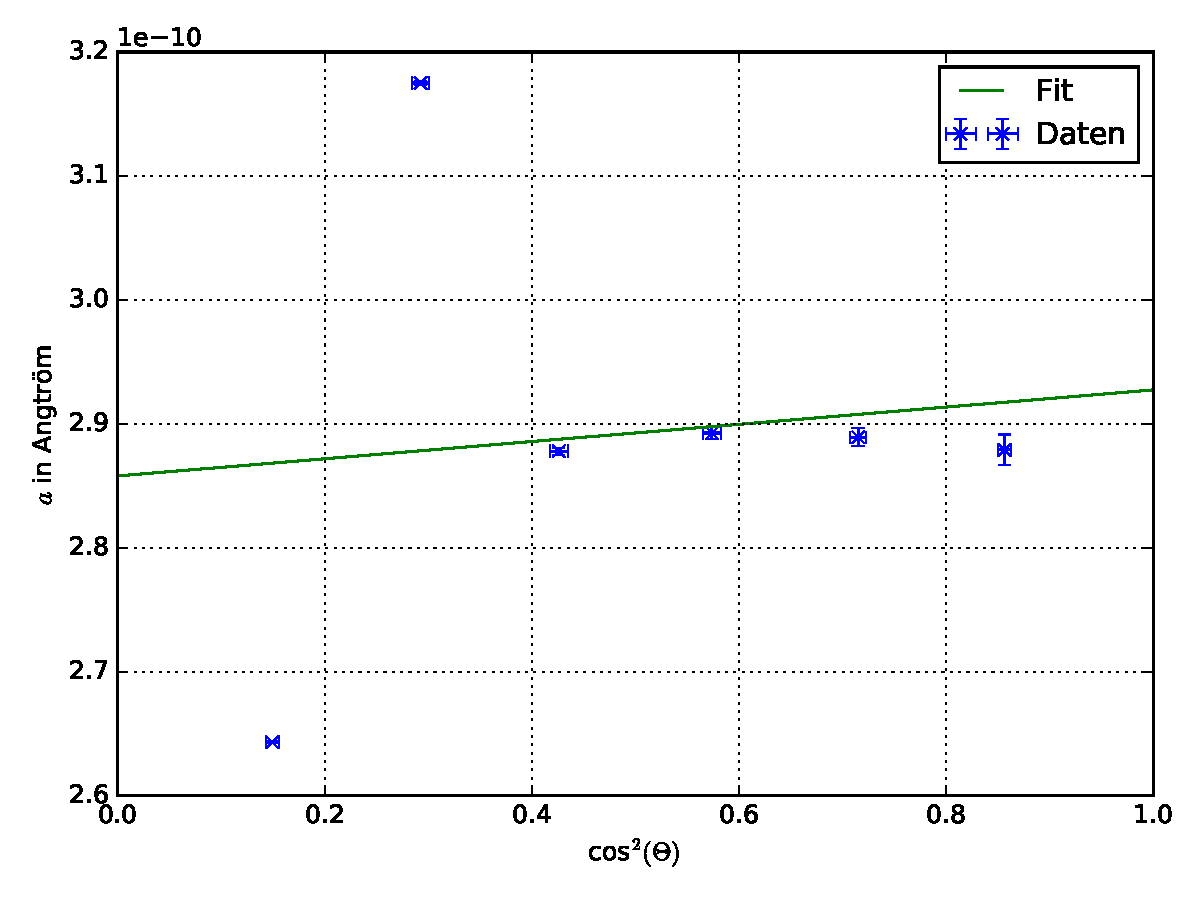
\includegraphics[width=\textwidth]{Abbildungen/Metall_Fit.pdf}
		\subcaption{Linearer Fit der Metall-Analyse um den systematischen Fehler durch die Verschiebung der Kristalle von der Achse zu eliminieren.}
		\label{fig:fit_metall}
	\end{minipage}
	\begin{minipage}[t]{0.45\textwidth}
		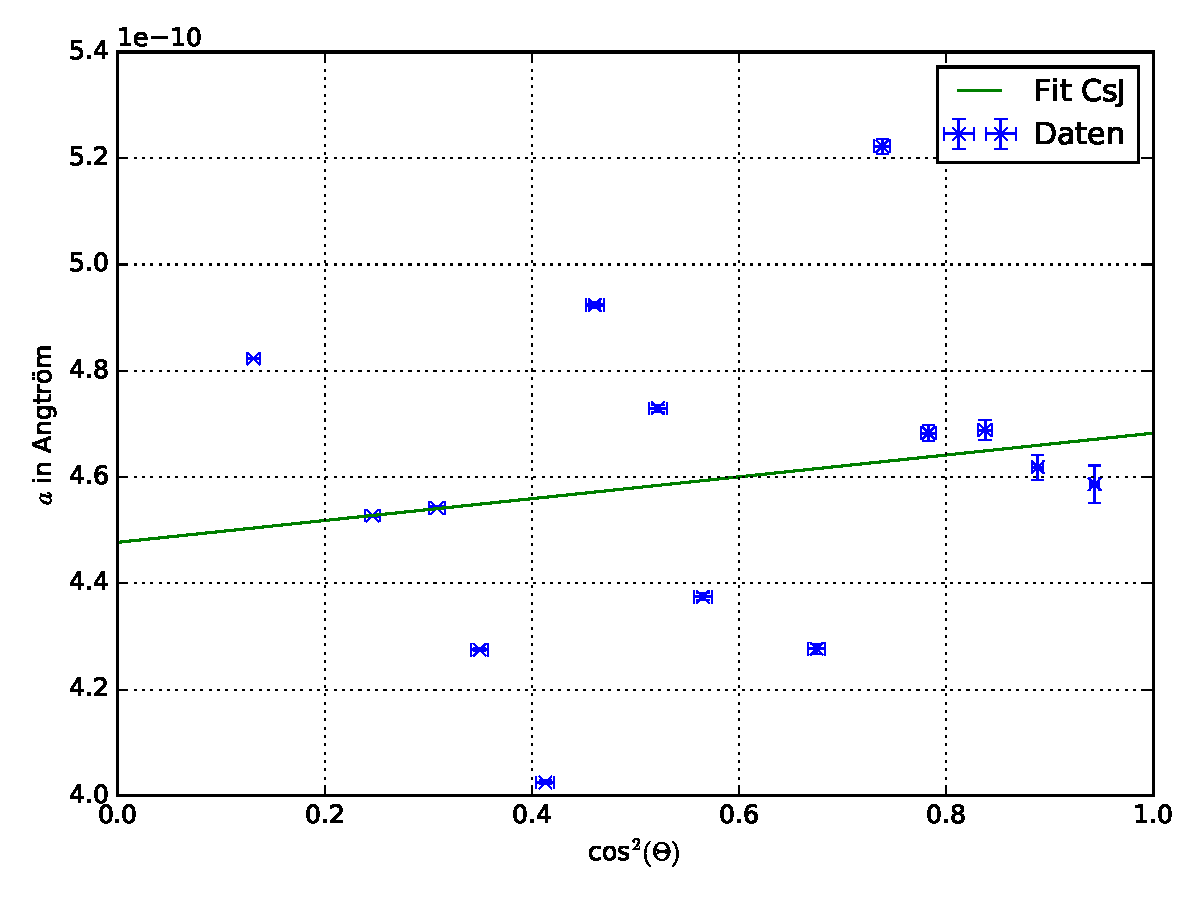
\includegraphics[width=\textwidth]{Abbildungen/Salz_Fit_Egor.pdf}
		\subcaption{Linearer Fit der Salz-Analyse um den systematischen Fehler durch die Verschiebung der Kristalle von der Achse zu eliminieren.}
		\label{fig:fit_salz}
\end{minipage}
% \caption{Die Elementaren kubischen Gittertypen bei denen gilt $|a|=|b|= |c|$. \cite{Anleitung}}
\end{figure}
>>>>>>> fürs erste fertig

\newpage
\section{Diskussion}
\label{sec:Diskussion}

Es ist die Struktur eines Metall- und eines Salz-Präparates bestimmt. Außerdem ist die Gitterkonstante der beiden Stoffe ermittelt. In Tabelle \ref{tab:disk} sind die Ergebnisse für beide Stoffe zusammengefasst. Es lässt sich vermuten, dass das Metallpulver aus Eisen (Fe) besteht. Die Salzstruktur scheint Caesiumiodid (CsJ) zu sein.
%
\begin{table}[h]
\centering
\caption{Die Struktur und Gitterkonstanten verglichen mit den Literaturwerte für das Metall- und Salz-Präparat.}
\label{tab:disk}
\begin{tabular}{c | c | c | c}
		\hline
		Material & $a^{exp}$ & $a^{lit}$ & Abweichung in \% \\
		\hline
		Fe & $\SI{2.86(18)e-10}{m}$ & $\SI{2.86e-10}{m}$ & $0\pm6$ \\
		CsJ & $\SI{4.48(20)e-10}{m}$ & $\SI{4.57e-10}{m}$ & $2\pm4$ \\
		\hline
\end{tabular}
\end{table}

\newpage
% \nocite{numpy}
% \nocite{scipy}
% \nocite{matplotlib}
% \nocite{uncertainties}

\printbibliography
\newpage
\section{Anhang}
\label{sec:Anhang}


\end{document}
